\documentclass[journal,conference]{IEEEtran}


% correct bad hyphenation here
\hyphenation{op-tical net-works semi-conduc-tor}
\usepackage{amsmath}
\usepackage{comment}
\usepackage{booktabs}
\usepackage{subfigure}
\usepackage{xcolor}
\usepackage{listings}
\lstset{
  basicstyle=\fontsize{9}{10}\selectfont\ttfamily,
  numbers=left,
  numberstyle= \tiny,
  keywordstyle= \color{ blue!70},
  commentstyle= \color{red!50!green!50!blue!50},
  frame=single,
  rulesepcolor= \color{ red!20!green!20!blue!20} ,
  escapeinside=``,
  xleftmargin=1.5em,xrightmargin=0em, aboveskip=1em,
  framexleftmargin=2em,
  showstringspaces=false,
  showtabs=false,
  breaklines=true
}
\lstdefinelanguage{Solidity}
{
  morekeywords={contract, mapping, address, uint, private, function, public, if, payable},
  morecomment=[l]{//},
  morestring=[b]"
}

\usepackage{multirow}
\usepackage{multicol}
\usepackage{lipsum}
\usepackage{mathtools}
\usepackage{cuted}
\usepackage[normalem]{ulem}
\useunder{\uline}{\ul}{}

\usepackage{amsmath}
\usepackage{extpfeil}
\usepackage{mathpartir}
\usepackage[mathscr]{eucal}

\usepackage{CJK}

\usepackage{algorithm}
\usepackage{algorithmicx}
\usepackage{algpseudocode}
\renewcommand{\algorithmicrequire}{\textbf{Input:}}
\renewcommand{\algorithmicensure}{\textbf{Output:}}

\usepackage{hyperref}
\usepackage{cleveref}
\crefformat{section}{\S#2#1#3} % see manual of cleveref, section 8.2.1
\crefformat{subsection}{\S#2#1#3}
\crefformat{subsubsection}{\S#2#1#3}

\begin{document}
%
% paper title
% Titles are generally capitalized except for words such as a, an, and, as,
% at, but, by, for, in, nor, of, on, or, the, to and up, which are usually
% not capitalized unless they are the first or last word of the title.
% Linebreaks \\ can be used within to get better formatting as desired.
% Do not put math or special symbols in the title.
\title{Bare Demo of IEEEtran.cls for Journals}
%
%
% author names and IEEE memberships
% note positions of commas and nonbreaking spaces ( ~ ) LaTeX will not break
% a structure at a ~ so this keeps an author's name from being broken across
% two lines.
% use \thanks{} to gain access to the first footnote area
% a separate \thanks must be used for each paragraph as LaTeX2e's \thanks
% was not built to handle multiple paragraphs
%

\author{
	Zhongye~Wang,~\IEEEmembership{SJTU,}
	Jingyu~Li,~\IEEEmembership{SJTU,}
	Xiaoyi~Bao,~\IEEEmembership{SJTU,}
	Shangning~Xu,~\IEEEmembership{SJTU,}
	and Chenxuan~Li,~\IEEEmembership{SJTU}
}

% The paper headers
\markboth{Journal of \LaTeX\ Class Files,~Vol.~13, No.~9, September~2014}%
{Shell \MakeLowercase{\textit{et al.}}: Bare Demo of IEEEtran.cls for Journals}
% The only time the second header will appear is for the odd numbered pages
% after the title page when using the twoside option.
%
% *** Note that you probably will NOT want to include the author's ***
% *** name in the headers of peer review papers.                   ***
% You can use \ifCLASSOPTIONpeerreview for conditional compilation here if
% you desire.


% make the title area
\maketitle

% As a general rule, do not put math, special symbols or citations
% in the abstract or keywords.
\begin{abstract}
The abstract goes here.
\end{abstract}

% Note that keywords are not normally used for peerreview papers.
\begin{IEEEkeywords}
IEEEtran, journal, \LaTeX, paper, template.
\end{IEEEkeywords}


\IEEEpeerreviewmaketitle



\section{Introduction}
\IEEEPARstart{T}{his}

\section{Related Work}
% lcx
\section{Subsampling and Interpolation}

\subsection{Subsampling}
Resampling using pixel area relation. Suppose $x\times y$ image subsampled down to size $x'\times y'$. scale\_x = x/x', scale\_y = y/y', and then we get block $scale\_x \times scale\_y$, block\_area = $scale\_x \times scale\_y$, the new image's each pixel is the weighted average of pixels in corresponding block's of the original image: 
\begin{align*}
	p'(x',y')=\sum_{i,j}{\frac{covered\_area \cdot p(i,j)}{block\_area}}
\end{align*}
i,j are nonnegative integers, $i \in [scale\_x\times x,scale\_x\times (x+1)]$ $j \in [scale\_y\times y,scale\_y\times (y+1)]$

\subsection{Interpolation}
In the mathematical field of numerical analysis, interpolation is a type of estimation, a method of constructing new data points within the range of a discrete set of known data points. In this project we use bilinear interpolation, bicubic interpolation, Lanczos resampling.

\subsubsection{Bilinear Interpolation}
\begin{figure}[h]
	\centering
	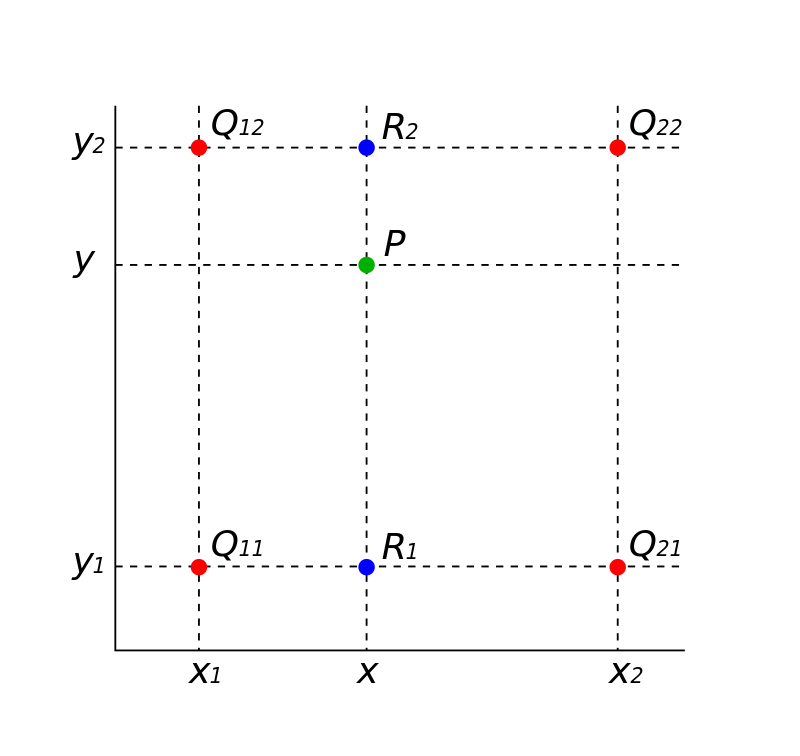
\includegraphics[width=0.6\linewidth]{fig/1.png}
	\label{fig:Bilinear Interpolation}
\end{figure}
\par First do linear interpolation in the x-direction:
\begin{align*}
p(R_1) = \frac{x_2-x}{x_2-x_1}\cdot p(Q_{11})+\frac{x-x_1}{x_2-x_1}\cdot p(Q_{21})\\
p(R_2) = \frac{x_2-x}{x_2-x_1}\cdot p(Q_{12})+\frac{x-x_1}{x_2-x_1}\cdot p(Q_{22})
\end{align*}
Then interpolate in the y-direction:
\begin{align*}
p(P) &= \frac{y2-y}{y2-y1}\cdot p(R_1)+\frac{y-y1}{y2-y1}\cdot p(R_2)\\ &=\small{\frac {1}{(x_{2}-x_{1})(y_{2}-y_{1})}}{\begin{bmatrix}x_{2}-x&x-x_{1}\end{bmatrix}}{\begin{bmatrix}f(Q_{11})&f(Q_{12})\\f(Q_{21})&f(Q_{22})\end{bmatrix}}{\begin{bmatrix}y_{2}-y\\y-y_{1}\end{bmatrix}}
\end{align*}
\par We can get the corresponding pixel's coordinate in original image: $x'\cdot scale\_x=x$, $y'\cdot scale\_y=y$. If either x or y is not integer, $x_1=int(x),x_2=int(x)+1,y_1=int(y), y_2=int(y)+1$, do interpolation.
\par This algorithm reduces some of the visual distortion caused by resizing an image to a non-integral zoom factor.
~\\
\subsubsection{Bicubic Interpolation}
~\\
\par In this method, new image’s pixel at point (x', y'), p(x',y'), is the weighted average of the nearest 16 points in the original image. An interpolator can be obtained by applying a convolution with the following kernel in both dimensions:
\begin{align*}
{\displaystyle W(x)={\begin{cases}(a+2)|x|^{3}-(a+3)|x|^{2}+1&{\text{for }}|x|\leq 1,\\a|x|^{3}-5a|x|^{2}+8a|x|-4a&{\text{for }}1<|x|<2,\\0&{\text{otherwise}},\end{cases}}}
\end{align*}
where a is usually set to −0.5 or −0.75.
\par $x'\cdot scale\_x=x$, $y'\cdot scale\_y=y$. If either x or y is not integer, $x_i$=int(x+i), $y_j$=int(y+j), i, j = -1,0,1,2:

do interpolation in the x-direction:
\begin{align*}
p(x',y_j)=\sum_{i}{W(x-x_i)\cdot p(x_i,y_j)}
\end{align*}
then do interpolation in the y-direction:
\begin{align*}
p(x',y')=\sum_{j}{W(y-y_j)\cdot p(x',y_j)} 
\end{align*}
\par Images resampled with bicubic interpolation are smoother and have fewer interpolation artifacts.
~\\
\subsubsection{Lanczos Resampling}
~\\
\par The effect of each input sample on the interpolated values is defined by the filter's reconstruction kernel L(x), called the Lanczos kernel. 
\begin{align*}
{\displaystyle L(x)={\begin{cases}\operatorname {sinc} (x)\,\operatorname {sinc} (x/a)&{\text{if}}\ -a<x<a,\\0&{\text{otherwise}}.\end{cases}}}
\end{align*}
Equivalently,
\begin{align*}
{\displaystyle L(x)={\begin{cases}1&{\text{if}}\ x=0,\\{\dfrac {a\sin(\pi x)\sin(\pi x/a)}{\pi ^{2}x^{2}}}&{\text{if}}\ -a\leq x<a\ {\text{and}}\ x\neq 0,\\0&{\text{otherwise}}.\end{cases}}}
\end{align*}
\par The parameter $a$ is a positive integer, typically 2 or 3 (but in opencv, the method is cv2.INTER$\_$LANCZOS4, $a$=4), which determines the size of the kernel. The Lanczos kernel has $2a-1$ labes:a positive one at the center, and $a-1$ alternating negative and positive lobes on each side.
\begin{align*}
L(x,y) &= L(x) \cdot L(y)\\
p(x',y') &= \sum_{i,j}{L(x_i-x)\cdot L(y_j-y)\cdot p(x_i,y_j)}
\end{align*}
$x_i=int(x+i)$, $y_j=int(y+j)$, $-a+1\leq i, j \leq a-1$

\section{Methodology}
In this section, we illustrate the concept and ideas behind our method of discriminating fake UHD images.
We start with a naive thinking about fabrication of UHD images, and based on the idea of reference in it, we develop the concept of relative DCT analysis and the energy spectrum analysis of the RDCT.


\subsection{A Naive Thought: Enumerative Search}
\cref{sec:enumerative}
We first try to tackle the problem with a very naive approach.
If we know all possible ways to generate false UHD images, assuming the number of them is limited, we can actually enumerate through all of them to determine which algorithm is applied in any given false UHD image.

We can do this by first subsampling a given image, then using every know algorithm to upsampling the downsampled image back to the original size.
Say the image is originally faked with algorithm A, then the reconstructed image using algorithm A should result in very small MSE wrt. to the original one.
If after enumerated all possible algorithms and subsampling rate (also assumed limited), no algorithm satisfy the above statement, then we can assert that the image is UHD.

The naive algorithm to determine the authenticity of an UHD image is however impractical and inefficient, because we cannot enumerate all possible ways to fabricate false UHD images and upsampling rate.
The application of DNN in UHD image generation also makes such approach infeasible due to tremendous amount of hyper-parameters to it.

However, we can still refer to the idea of reconstruct a reference image by first subsampling then upsampling with some reference interpolation method.
If we use the most trivial interpolation method to generate the reference, for any given image, the more it improves from the reference, we are more confident that it is true UHD.
This idea gives birth to the relative DCT analysis we propose later.

\subsection{Relative DCT Analysis of UHD Images}
The are natural differences between real UHD images and fake UHD image generated with interpolation.
Real UHD images contains large amount of real objects, each with some random but distinct characteristics.
Therefore, if we use functions to fit pixel values in different regions, there should be very few similarities between those functions.
On the other hand, because it is often a common practice to use a single interpolation function to do upsampling to get fake UHD images, the functions in different regions should share certain similarities.
Some interpolation methods (like bicubic) would even result in same family of those functions.

Another idea is that, there are always noises in real UHD images due to the inherent deficiencies in equipments, whereas the fake UHD images undergoes a stage of subsampling, which eliminates some noises.
As a result, the fake UHD image should be more smooth than the original one.
We can use DCT to extract the magnitudes at different frequencies, and observe those for high frequencies is relatively lower in fake UHD images.

We goes with the latter approach, while the former one is more promising if we have efficient way to identify similarities between sampled values of functions.
Nevertheless, we need a way to extract features of those functions in both approaches, that is where discrete cosine transform (DCT) come into place.

\subsubsection{Relative DCT (RDCT) Analysis}
Different from traditional DCT analysis, we introduce the concept of relative DCT analysis based on the idea of reference image proposed in \ref{sec:enumerative}.
The DCT coefficients for the original image are given by \eqref{eq:dct}.
\begin{equation}
	\begin{array}{l}
		\mathcal{D}(u, v) = c(u)c(v)\sum_{x=0}^{N-1}\sum_{y=0}^{N-1}f(x, y)C(x, u)C(y, v)\\
		\vspace{-0.75em}\\
		\text{where } c(u) = \begin{cases}
			\sqrt{\frac{1}{N}} & u = 0 \\
			\sqrt{\frac{2}{N}} & u \neq 0
		\end{cases}, C(x, u) = \cos\bigg[\frac{(x+0.5)\pi}{N}u\bigg]
	\end{array}
	\label{eq:dct}
\end{equation}

We define the reference image $f'$ with downsampling rate $\alpha$ and upsampling method $p$ and its DCT coefficients $\mathcal{D}'$.
We then define the relative DCT transform in \eqref{eq:rel_dct}.
\begin{equation}
	\mathcal{D}_r(u, v) = \begin{cases}
		\frac{\mathcal{D}(u, v)}{\mathcal{D}'(u, v)} - 1 & \mathcal{D}'(u, v) \neq 0 \\
		\inf & \mathcal{D}'(u, v) = 0
	\end{cases}
	\label{eq:rel_dct}
\end{equation}
For any image, the relative DCT coefficients should give a fair criteria that is less sensitive to the content in the image.

\subsubsection{Tiled DCT Analysis} We also consider it more practical to apply DCT analysis on tiles of images instead of the entire one.
This is not only because it is faster and gives more stable and smaller DCT coefficients, but also due to the fact that the upsampling often considers only the region around the pixel to reconstruct.
For some tile width $T$, we define the $(i, j)$ tile of image in \eqref{eq:tile}.
\begin{equation}
	\begin{array}{l}
		f^{(i,j)}(x, y) = f(i * T + x, j * T + y), \\
		\vspace{-0.75em}\\
		\forall 0 \leq x, y < T, 0 \leq i, j < \min\{\lfloor\frac{W}{T}\rfloor, \lfloor\frac{H}{T}\rfloor\}
	\end{array}
	\label{eq:tile}
\end{equation}
We denote the relative DCT coefficients for the tile as $\mathcal{D}_r^{(i, j)}(u, v)$.

Figure~\ref{fig:rdct_hist} shows the distribution of RDCT coefficients with magnitudes less than 20 in tiles of a sample image, where we use a reference sampling rate of 2 and use the area average as a reference interpolation.

\begin{figure}[h]
	\centering
	\begin{minipage}{\linewidth}
		\subfigure[Histogram for Small RDCT Coefficients in a 4K Sample]{
			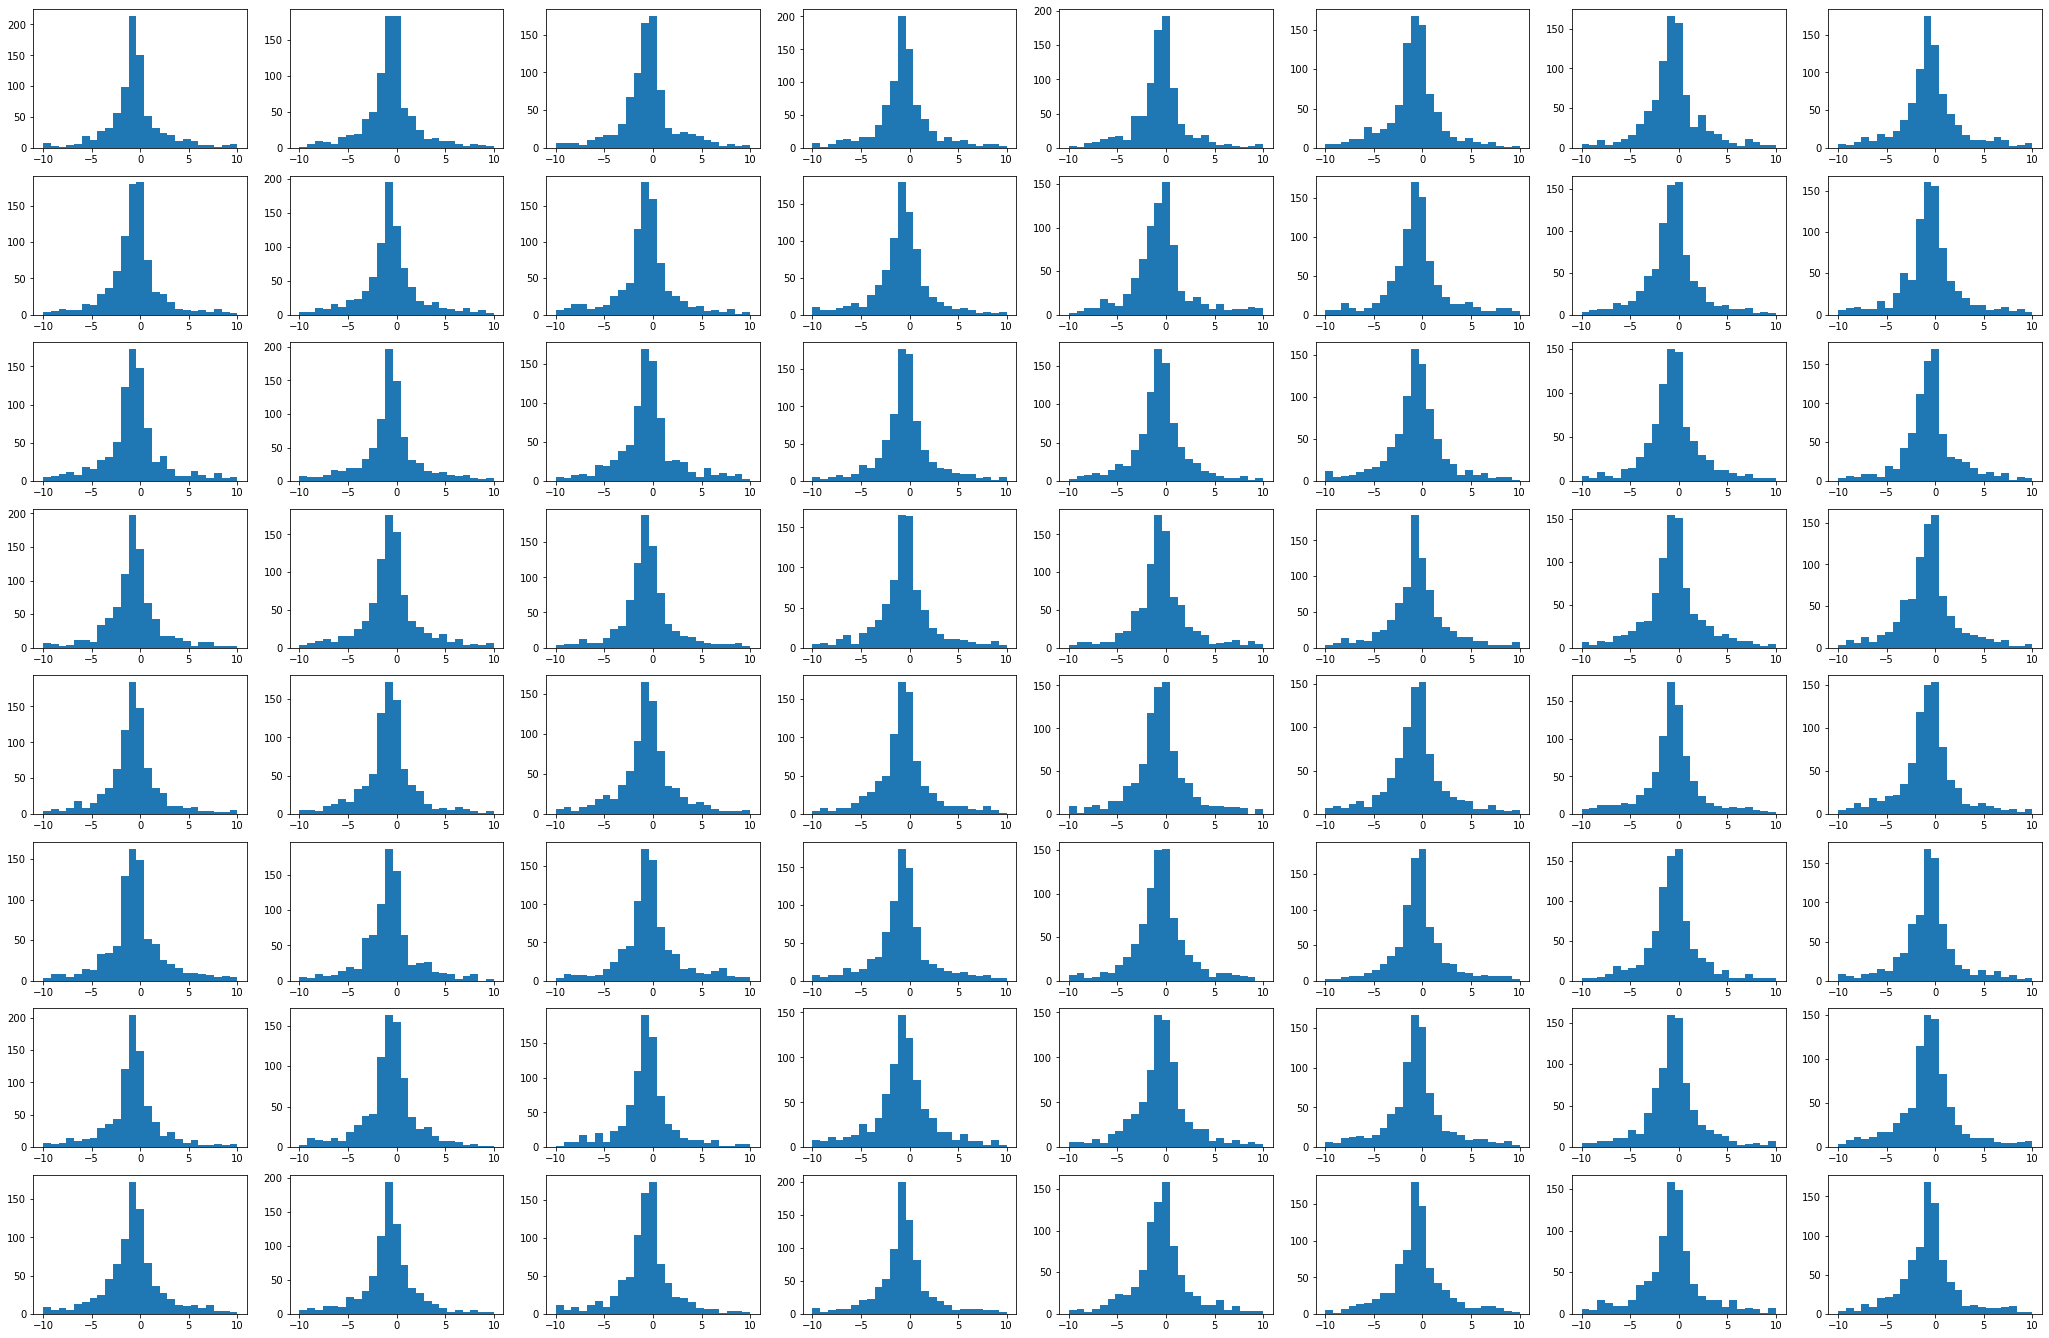
\includegraphics[width=\linewidth]{fig/rel_dct_hist_4k.png}
			\label{fig:rdct_hist_4k}
		}
	\end{minipage}
	\begin{minipage}{\linewidth}
		\subfigure[Histogram for Small RDCT Coefficients in an upsampled 1080P Sample]{
			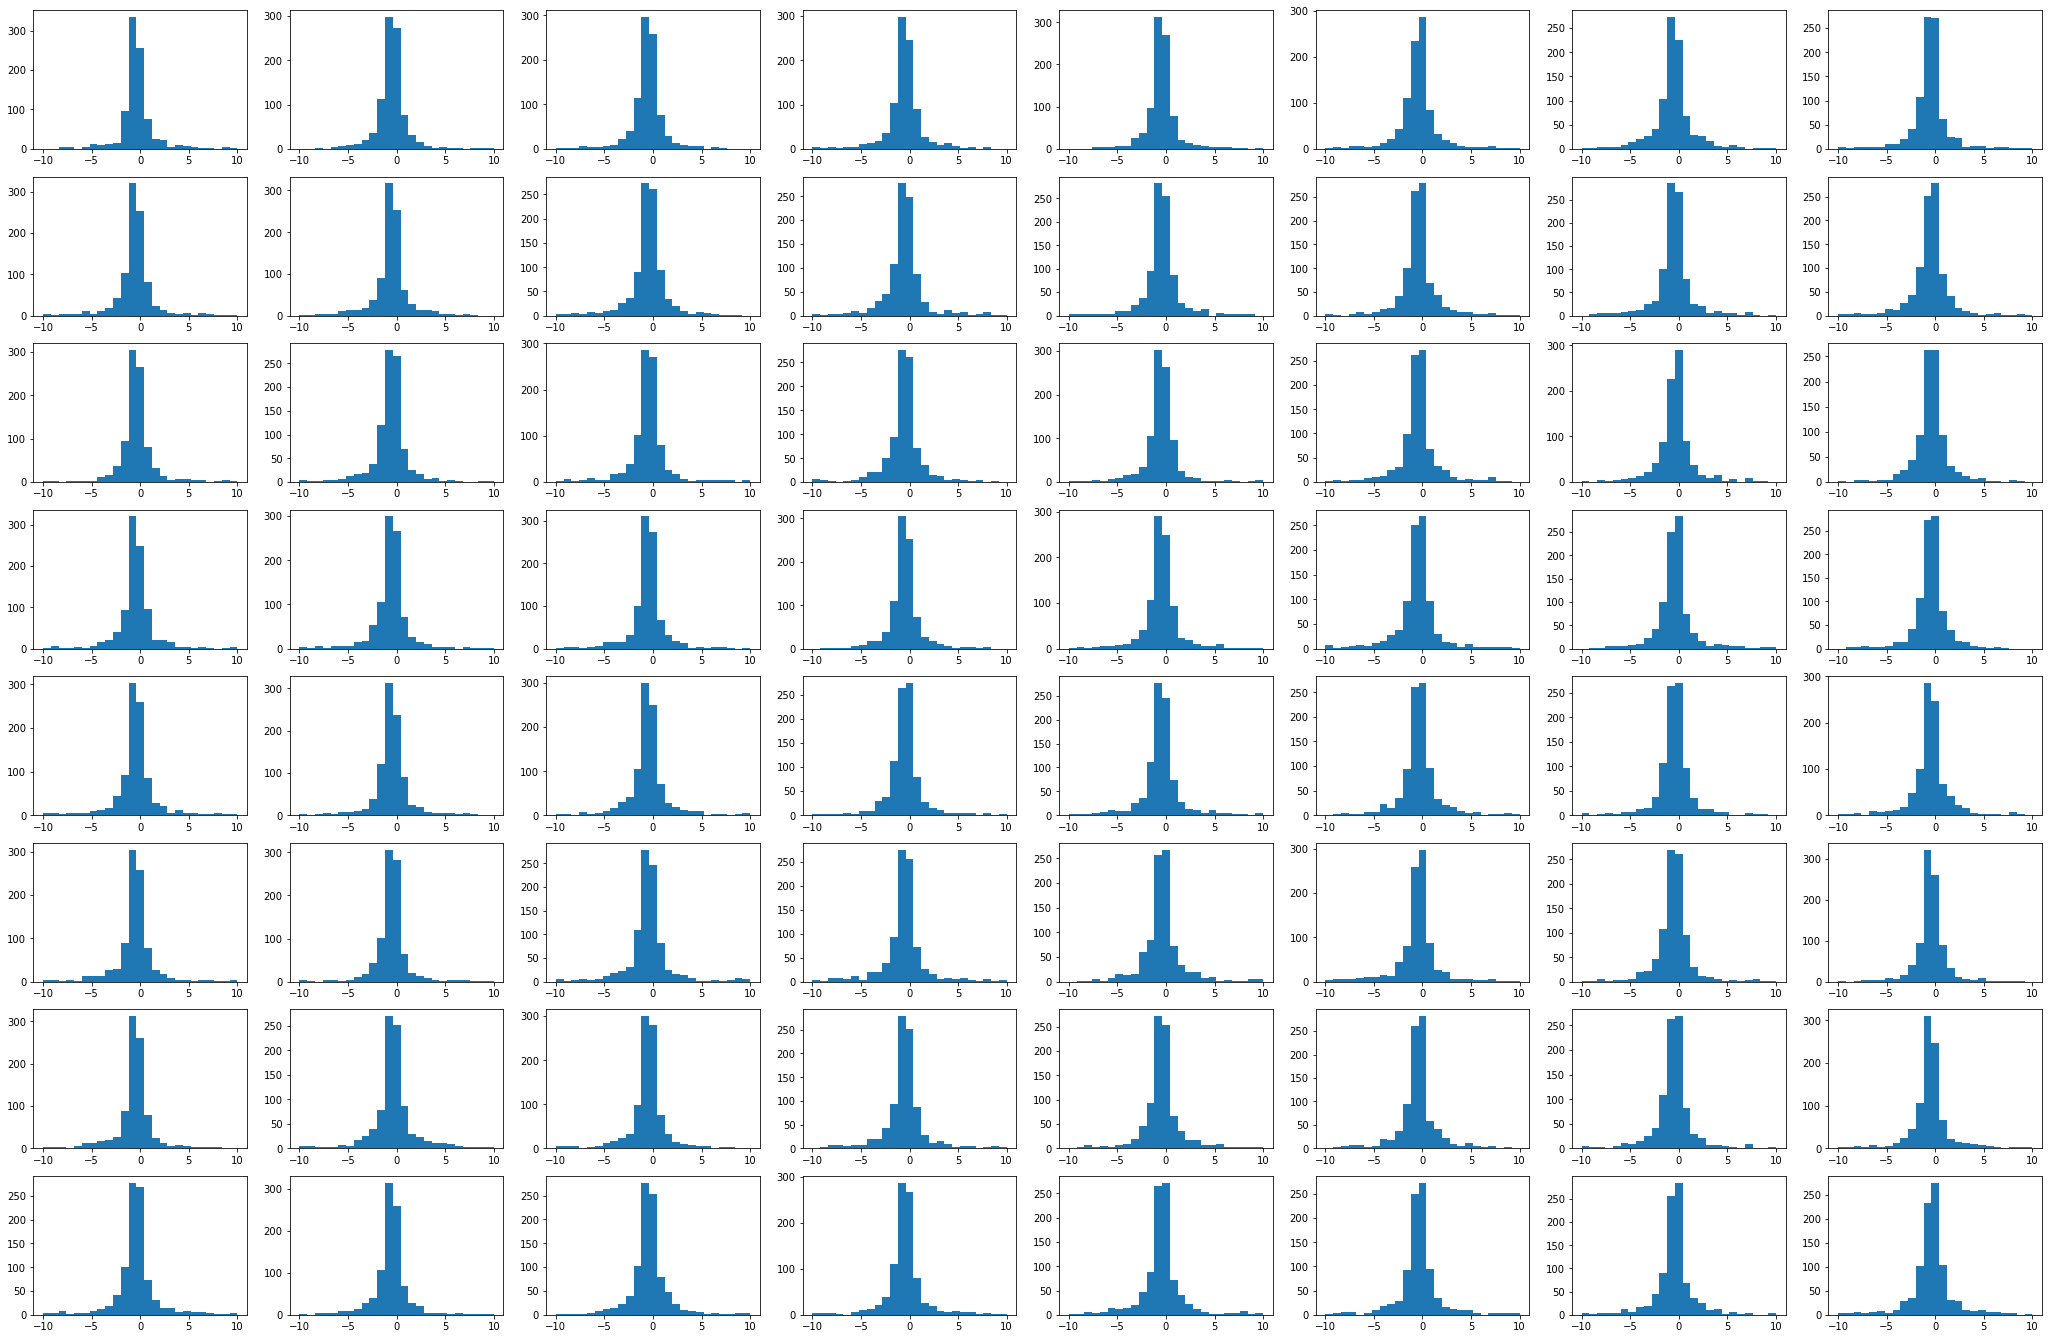
\includegraphics[width=\linewidth]{fig/rel_dct_hist_1080.png}
			\label{fig:rdct_hist_1080}
		}
	\end{minipage}
	\caption{Histograms for Small RDCT Coefficients in the 64 Tiles on the Upper-Left Corner of 1.bmp: The x-axis is the magnitudes of RDCT coefficients ranging from -20 to 20.}
	\label{fig:rdct_hist}
\end{figure}

\subsection{Relative Energy Spectrum}
We can observe the distributions of RDCT coefficients are more flat for the true 4K image in Figure~\ref{fig:rdct_hist_4k} than those in the fake, upsampled 1080P image in Figure~\ref{fig:rdct_hist_1080}, with the peaks in the latter appearing more sharp.

This phenomenon is actually prevalent not only in these tiles of the image, but also in most of tiles in all sample images.
We can interpolate it as follows:\begin{enumerate}
	\item The fake image become more smooth with value functions in different regions more unified towards the interpolation function. Therefore, some less relevant components (frequencies with small RDCT coefficients) will be suppressed in the fake, interpolated samples.
	\item This does not mean that the components with large magnitudes are also suppressed. In fact, most of them stays the same as those in the original image, because they compose the dominant content of the image.
\end{enumerate}

Based on this knowledge, we step further to calculate the average relative energy spectrum in tile $(i, j)$ using \eqref{eq:energy}.
\begin{equation}
	E_{L_2}^{(i, j)} = \int_{u,v} \big|\mathcal{D}_r^{(i, j)}(u, v)\big|^2 dudv \Big/ \int_{u,v} dudv
	\label{eq:energy}
\end{equation}

Figure~\ref{fig:ave-energy-hist} shows the average relative energy distribution for tiles in Figure~\ref{fig:rdct_hist}.
It is obviously that the relative energy of the real UHD tiles is higher than those of all upsampled tiles.

\begin{figure}[h]
	\centering
	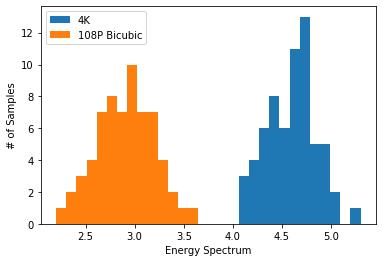
\includegraphics[width=0.99\linewidth]{fig/rel_energy_4k_1080.png}
	\caption{Histogram of Tile-Average Relative Energy Distribution}
	\label{fig:ave-energy-hist}
\end{figure}

To extract the average relative energy spectrum of an image, we can either compute the average of all tile-average energy spectrum of all tiles of the image, or more efficiently, only compute those for randomly sampled tiles.
In following experiments, we will go with the later one.

This gives us a preferable criteria to discriminate real and fake UHD image using relative DCT and energy spectrum analysis.
We will then examine other ways of constructing the reference image and calculating the energy spectrum.

\section{Experiments}
In this section, we build upon previous concepts to test different methods of discriminating fake UHD images.

\subsection{A Simple Thresholding Method}
We first extract the $L_1$ and $L_2$ relative energy spectrum of all images, with sampling rate 2 and area average interpolation as the reference.
The $L_1$ spectrum is defined by \eqref{eq:l1-energy}.
\begin{equation}
	E_{L_1}^{(i, j)} = \int_{u,v} \big|\mathcal{D}_r^{(i, j)}(u, v)\big| dudv \Big/ \int_{u,v} dudv
	\label{eq:l1-energy}
\end{equation}

The average energy spectrums of all 200 images, with their original 4K resolution, and fabrication upsampled from 720P and 1080P with bicubic, bilinear, and lanzcos2 interpolation, are shown in Figure~\ref{fig:rel-energy-spec}.

\begin{figure}[h]
	\centering
	\begin{minipage}{0.95\linewidth}
		\subfigure[$L_1$ Energy Spectrum and Threshold]{
			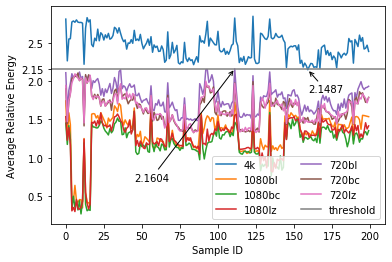
\includegraphics[width=\linewidth]{fig/threshold_L1.png}
		}
	\end{minipage}
	\begin{minipage}{0.95\linewidth}
		\subfigure[$L_2$ Energy Spectrum and Threshold]{
			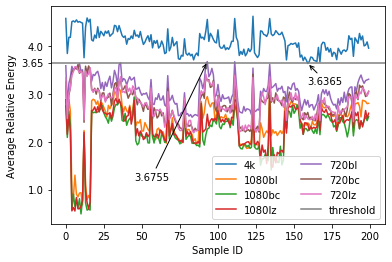
\includegraphics[width=\linewidth]{fig/threshold_L2.png}
		}
	\end{minipage}
	\caption{Relative Energy Spectrum of all 1400 Samples}
	\label{fig:rel-energy-spec}
\end{figure}

We can easily distinguish between the energy spectrum of real 4K images and fake ones, where the curve for real ones occupy the higher part, while that of fake ones occupy the low part.
We calculate the threshold that divides two groups using the binary search depicted in Algorithm~\ref{alg:binary-search}.
In this case, it is exactly the average of the minimum energy spectrum value of the real ones (sample 160.bmp) and the maximum energy spectrum value of the fake ones (sample 112.bmp (720P bilinear) in $L_1$ and sample 94.bmp (720P bilinear) in $L_2$).
We mark two thresholds with grey lines and those critical points in Figure~\ref{fig:rel-energy-spec}.

\begin{algorithm}[h]
	\caption{Binary Search: A heuristic search for the optimal threshold minimizing total mistakes.}
	\label{alg:binary-search}
	\begin{algorithmic}
		\Require The average energy spectrum of 200 true UHD images and 1200 fake UHD images.
		\Ensure The threshold value.
		\State $high \leftarrow \text{maximum energy spectrum in fake UHD images};$
		\State $low \leftarrow \text{minimum energy spectrum in true UHD images};$
		\State $best \leftarrow (low + high) / 2;$
		\While{$low + \epsilon < high$}
			\State Calculate the mistakes for positive and negative samples wrt. the current $mid$;
			\If{False negative is more then false positive}
				\State $low \leftarrow mid;$
			\Else
				\State $high \leftarrow mid;$
			\EndIf
			\If{The total mistakes for $mid$ are less than those for $best$}
				\State $best \leftarrow mid;$
			\EndIf
		\EndWhile
		\State \Return $best;$
	\end{algorithmic}
\end{algorithm}

We use these thresholds as criteria to judge the authenticity of a UHD image.
When the average relative energy is higher than the threshold, then we label it as a true UHD image.
Otherwise, we label it as a fake UHD image.
Table~\ref{tab:threshold-confusion-table} shows the confusion matrix of classification results for 1400 samples using $L_1$ criteria and $L_2$ criteria separately.
Both threshold models achieve remarkable accuracy.

\linespread{1.2}
\begin{table}[h]
	\centering
	\caption{Classification Result with Simple Thresholding}
	\label{tab:threshold-confusion-table}
	\begin{tabular}{|c|c|c|c|c|c|}
	\hline
	\multicolumn{2}{|c|}{\multirow{2}{*}{}} & \multicolumn{2}{c|}{L1 Prediction} & \multicolumn{2}{c|}{L2 Prediction} \\ \cline{3-6} 
	\multicolumn{2}{|c|}{}                  & Real             & Fake            & Real             & Fake            \\ \hline
	\multirow{2}{*}{Truth}      & Real      & 199              & 1               & 199              & 1               \\ \cline{2-6} 
								& Fake      & 1                & 1199            & 2                & 1198            \\ \hline
	\end{tabular}
\end{table}
\linespread{1.0}

We do realize that we are not testing the model on some hold-out set.
But the model is too simple to cause overfitting, making the validation unnecessary.
The quality of the threshold is desirable since it precisely splits the energy spectrums into two parts with no bias to any side.
Notice that taking out those critical points causing the threshold would result in dramatic downfall in the performance.
However, the critical points have already crossed the threshold and there are many other peak points centering around it, which means new data points will not have any meaningful improvements to the threshold.
Therefore, our method should be valid.

We also test the simple thresholding method on energy spectrum extracted using other reference interpolation and reference rate.
Table~\ref{tab:acc-ref-param} shows the accuracy for different parameter settings of the reference images.

\linespread{1.2}
\begin{table}[h]
	\caption{Accuracy for Different Reference Settings}
	\label{tab:acc-ref-param}
	\begin{tabular}{|c|c|c|c|c|c|}
	\hline
	\multicolumn{2}{|c|}{Parameters}                                                & \multicolumn{2}{c|}{L1 Accuracy}      & \multicolumn{2}{c|}{L2 Accuracy}      \\ \hline
	Ref Rate           & \begin{tabular}[c]{@{}c@{}}Ref\\ Method\end{tabular}       & Positive         & Negative           & Positive         & Negative           \\ \hline
	\multirow{4}{*}{2} & Area                                                       & \textbf{199/200} & \textbf{1199/1200} & \textbf{199/200} & 1198/1200          \\ \cline{2-6} 
					   & NN & \textbf{199/200} & \textbf{1199/1200} & \textbf{199/200} & \textbf{1199/1200} \\ \cline{2-6} 
					   & Bilinear                                                   & 196/200          & 1199/1200          & 191/200          & 192/200            \\ \cline{2-6} 
					   & Bicubic                                                    & 179/200          & 1178/1200          & 168/200          & 167/200            \\ \hline
	3                  & Area                                                       & 153/200          & 1190/1200          & 155/200          & 1188/1200          \\ \hline
	\end{tabular}
\end{table}
\linespread{1.0}

The simplest reference interpolations, the area average and nearest neighbors, achieves the best performance, which confirms our conjecture that the reference is the baseline for the improvements of image quality.

\subsection{Joint Feature and SVM}
In the previous experiments, although larger reference rate causes dramatic performance drop, we know from the visualization that the gap between the energy of true UHD images and fake UHD images varies greatly on some samples.
Some gaps emerge in other reference method are absent from the area average and nearest neighbors ones.
Therefore, we see the possibility of combining all possible average relative energy spectrums for one image into a feature of it, and apply traditional machine learning method to obtain a model for the joint feature.

We select all 5 reference methods presented in Table~\ref{tab:acc-ref-param} along with the raw DCT energy spectrum, which is 12 features in total.
After concatenating all features together into 10-dimensional vectors, we first apply principle component analysis to have a glance at the data distribution.
Figure~\ref{fig:pca} shows the PCA visualization, from which we are sure there exists a efficient way to separate all true and fake UHD images.

\begin{figure}[h]
	\centering
	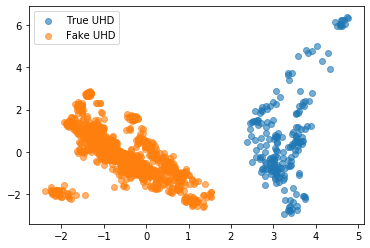
\includegraphics[width=0.95\linewidth]{fig/pca.png}
	\caption{PCA Visualization of all 12 Features}
	\label{fig:pca}
\end{figure}

We apply the support vector machine classifier with RBF kernel and train the classifier on 43 positive samples and 237 negative samples and validate it on the rest 1120 samples.
The SVM classifier achieves 100\% accuracy on both the training set and validation set.

\subsection{Test Models on DNN Generated Images}
We have previously ignored the fake UHD images generated with DNNs like SRCNN and EDSR, and now we use them to test and improve the models we have proposed.

We first observe that the simple thresholding methods with area average reference and nearest neighbor reference still work for the fake UHD images generated with EDSR, while they fail dramatically for those generated with SRCNN.
The performance for SVM using the joint feature also drops greatly encountering DNN generated images.
Table~\ref{tab:acc-test} shows the accuracies for those methods.

\linespread{1.2}
\begin{table}[h]
	\caption{Accuracy for Different Methods on DNN Generated Test Set}
	\label{tab:acc-test}
	\begin{tabular}{|c|c|c|c|c|c|c|}
		\hline
		 & \multicolumn{4}{c|}{Simple Thresholding} & \multirow{2}{*}{\begin{tabular}[c]{@{}c@{}}Joint\\ Feature\\ SVM\end{tabular}} & \multirow{2}{*}{\begin{tabular}[c]{@{}c@{}}Partially\\ Retrained\\ SVM\end{tabular}} \\ \cline{1-5}
		\begin{tabular}[c]{@{}c@{}}DNN Type\\ \& Defintion\end{tabular} & AR L1 & AR L2 & NN L1 & NN L2 &  &  \\ \hline
		SRCNN 1080P & 68\% & 55\% & \textbf{68.5\%} & 53.5\% & 46\% & {\ul \textbf{97\%}} \\ \hline
		SRCNN 720P & 62.5\% & \textbf{63.5\%} & 60\% & 62.5\% & 37.5\% & {\ul \textbf{93.5\%}} \\ \hline
		EDSR 1080P & {\ul \textbf{100\%}} & {\ul \textbf{100\%}} & {\ul \textbf{100\%}} & {\ul \textbf{100\%}} & 94.5\% & {\ul \textbf{100\%}} \\ \hline
		EDSR 720P & 95.5\% & \textbf{96.5\%} & \textbf{96.5\%} & 96\% & 93.5\% & {\ul \textbf{100\%}} \\ \hline
	\end{tabular}
\end{table}
\linespread{1.0}

This clearly shows the advantage of SRCNN over EDSR wrt. the ability to simulate real UHD images.
We add the DNN generated samples onto the previous PCA visualization in Figure~\ref{fig:pca-dnn}.
We can see that the DNN samples fills in exactly the gap between the interpolation generated samples and true UHD images, which causes the drop of the performance for various methods.
However, this means we can also improve the performance at least for SVM by including some DNN generated samples into the training set, because the separation between true UHD samples and fake ones is still clear.

\begin{figure}[h]
	\centering
	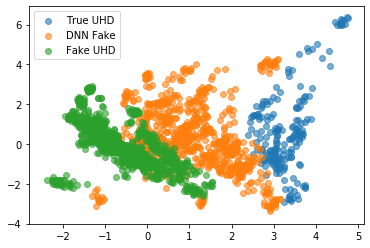
\includegraphics[width=0.95\linewidth]{fig/pca_dnn.png}
	\caption{PCA Visualization with DNN Fake Samples}
	\label{fig:pca-dnn}
\end{figure}

We combine the DNN generated samples with interpolated ones, and train a SVM model on 10\% of those samples with 97.7\% accuracy on the 10\% training set and 96.6\% accuracy on the 90\% training set.
The accuracy of this partially trained model for different DNN fake images classification is shown in the last column of Table~\ref{tab:acc-test}.


\section{Conclusion}
In this project, we explore the potential for DCT analysis on classifying true UHD images and fabricated ones by proposing the concept of reference and relative DCT analysis.
We analyze the sampled energy spectrums of the relative DCT coefficients of a images and apply a simple thresholding method and SVM to perform the binary classification task.
The simple thresholding requires very computation of features while the SVM provides stable performance even on DNN generated samples.

In our application, we offer a simple thresholding model with area average reference and a SVM model trained on homebrew fake UHD images using both interpolation and DNN generation.



\bibliographystyle{IEEEtran}
\bibliography{Ref}


% that's all folks
\end{document}